\documentclass[12pt,a4paper]{article}
\usepackage[utf8]{inputenc}
\usepackage[french]{babel}
\usepackage[T1]{fontenc}
\usepackage{amsmath}
\usepackage{amsfonts}
\usepackage{amssymb}
\usepackage{makeidx}
\usepackage{graphicx}
\usepackage{lmodern}
\usepackage{index}
%\usepackage{hyperref}
\newcommand{\HRule}{\rule{\linewidth}{0.5mm}}
%\usepackage{kpfonts}
\usepackage{fourier}
\usepackage[left=2cm,right=2cm,top=2cm,bottom=2cm]{geometry}
\author{Sarah Kaddah}
\title{Rapport de stage}

%%%%%%%%%%Interligne
\renewcommand{\baselinestretch}{1.5}
\begin{document}
%%%%%%%%%%%%%%%%%%%%%%%%%%%%%%%%%%%%%%%%%%%%%%%%%%%%%%%%%%%%%%%%%
%%%%%%%%%%%%%%%%%%%%%%1ere page%%%%%%%%%%%%%%%%%%%%%%%%%%%%%%%%%%
%%%%%%%%%%%%%%%%%%%%%%%%%%%%%%%%%%%%%%%%%%%%%%%%%%%%%%%%%%%%%%%%%
%%%%%%%%%%%%%%%%%%%%%%%%%%%%%%%%%%%%%%%%%%%%%%%%%%%%%%%%%%%%%%%%%
\begin{titlepage}
  \begin{sffamily}
  \begin{center}
	\large{Master 2 Biologie-Informatique/ Bioinformatique \hfill 2017-2018}
	\flushleft{\large{Université Paris Diderot - Paris 7}}
	
%	\begin{center}
%		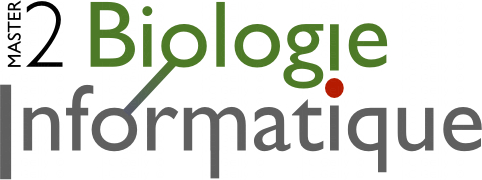
\includegraphics[scale=0.3]{img/m2.png} \hfill
%		
\includegraphics[scale=0.1]{img/p7.png}
%	\end{center}

\begin{tabular}{c}
\\ \\ \\
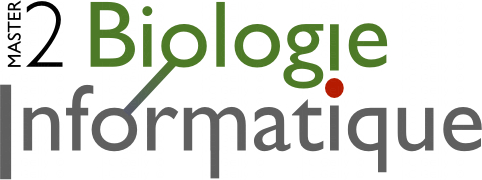
\includegraphics[scale=0.3]{img/m2.png}
\end{tabular}
\hfill
\begin{tabular}{c}
\\

\includegraphics[scale=0.1]{img/p7.png}
\end{tabular}

%%%%%%%%% Title    
    \HRule \\[0.2cm]
    { \huge \bfseries \center{Etude de la fonction et des mécanismes d'évolution des séquences répétées centromériques chez les Primates}\\[0.4cm] }
    \HRule \\[2cm]
%%%%%%%%Centre de la page    
\begin{center}\LARGE{\textbf{Sarah Kaddah}}\end{center}
\begin{center}\Large{Tuteur: Lo\"{i}c Ponger}\end{center}~\\[0.5cm]
%%%%%%%%% Bottom of the page
\center{\large{Structure et Instabilité des Génomes}}
\center{\large{ MNHN - CNRS UMR 7196 / INSERM U1154 - Sorbonne Universités}}\\[1cm]

%	\begin{center}
%		
\includegraphics[scale=0.2]{img/mnhn.jpg} \hfill
%		
\includegraphics[scale=0.08]{img/cnrs.png} \hfill
%		
\includegraphics[scale=0.08]{img/inserm.jpg}
%	\end{center} 

\begin{tabular}{cc}
 \hspace*{3cm} &  

\includegraphics[scale=0.2]{img/mnhn.jpg}
\end{tabular}
\hfill
\begin{tabular}{c}

\includegraphics[scale=0.08]{img/inserm.jpg}
\end{tabular}
\hfill
\begin{tabular}{cc}

\includegraphics[scale=0.08]{img/cnrs.png} &
\hspace*{3cm}
\end{tabular}

%%%%%%%%% END
  \end{center}
  \end{sffamily}
\end{titlepage}
%%%%%%%%%%%%%%%%%%%%%%%%%%%%%%%%%%%%%%%%%%%%%%%%%%%%%%%%%%%%%%%%%%
%%%%%%%%%%%%%%%%%%%%%Remerciements%%%%%%%%%%%%%%%%%%%%%%%%%%%%%%%%
%%%%%%%%%%%%%%%%%%%%%%%%%%%%%%%%%%%%%%%%%%%%%%%%%%%%%%%%%%%%%%%%%%
\thispagestyle{empty}
\section*{\begin{center}Remerciements\end{center}}~\\[0.2cm]
\addcontentsline{toc}{section}{Remerciements}
Merci à Namrod pour toute la partie sur la bibliographie. Retrouvez ses questions FAQ qui ont permis la rédaction de cette partie.\\
\noindent Merci à f-leb, LittleWhite et Metalman pour leurs conseils et la relecture.
\noindent Merci à ced et jacques\_jean pour la correction orthographique et typographique.


%%%%%%%%%%%%%%%%%%%%%%%%%%%%%%%%%%%%%%%%%%%%%%%%%%%%%%%%%%%%%%%%%%
%%%%%%%%%%%%%%%%%%%Table des matières%%%%%%%%%%%%%%%%%%%%%%%%%%%%
%%%%%%%%%%%%%%%%%%%%%%%%%%%%%%%%%%%%%%%%%%%%%%%%%%%%%%%%%%%%%%%%%

\newpage
\tableofcontents
\setcounter{page}{0}
\newpage 
%%%%%%%%%%%%%%%%%%%%%%%%%%%%%%%%%%%%%%%%%%%%%%%%%%%%%%%%%%%%%%%%
%%%%%%%%%%%%%%%%%%%%Introduction%%%%%%%%%%%%%%%%%%%%%%%%%%%%%%%%
%%%%%%%%%%%%%%%%%%%%%%%%%%%%%%%%%%%%%%%%%%%%%%%%%%%%%%%%%%%%%%%% 

\section{Introduction}
\subsection{Les séquences centromériques}
-> biblio CENP-A\\
-> biblio kinetochore\\
-> info supp sur l'ADN satellite\\

Le centromère est une structure chromatinienne caractérisé par la présence de CENP-A. Cette protéine, très conservée au cours de l'évolution, est un variant de l'histone H3. Son rôle est de fixer la position du kinétochore par un mécanisme encore peu connu. En effet, le centromère est le site d'assemblage du kinétochore, un ensemble d'ADN et de protéines. Il permet l'attachement du fuseau mitotique pour la ségrégation des chromosomes durant la division cellulaire chez les eucaryotes. Le centromère et les protéines impliquées sont relativement bien conservés. Au contraire, l'ADN sous-jacent est très diversifié et l'organisation varie d'un taxon à l'autre. Cependant, une caractéristique commune est retrouvée chez toute les espèces: de l'ADN centromérique répété en tandem nommé ADN satellite. Ces répétitions sont issues d'événements d'amplification, tels les crossovers inégaux, la conversion de gènes, les cercles roulants ou la transposition de séquences.[Malik and Henikoff, 2002; Plohl et al. 2012]
Ces séquences représentent 5\% du génome. Les répétitions s'étendent de 7pb à 3,2kb avec des séquences de 145-180kb le plus souvent.  

\subsection{L'ADN $\alpha$-satellites}
-> première mise en évidence des AS\\
->théorie gradient de l'âge\\
-> travaux sur le gorille à dev\\

L'ADN satellite chez les Primates est connu sous le nom d'$\alpha$-satellite. Ces séquences centromériques répétées en tandem sont riches en AT. 
-> article sur la première découverte

Des études chez l'Homme propose un modèle évolutif. La répartition des $\alpha$-satellites suivrait une répartition spécifique selon l'âge des familles. Les familles les plus jeunes s'insèrent au cœur du centromère, repoussant les familles les plus anciennes jusqu'aux regions voisines, appelé péri-centromère.\\
->Article Shepelev\\
->Est-ce que je peux utiliser du conditionnel? OU est-ce que cette théorie est confirmée?

Un monomère a une longueur de 171pb et il peut être répété des milliers de fois. Les monomères peuvent être répartis en famille selon leur similarité, les séquences ayant un taux d'identité supérieur à 70\%. Ces séquences ont soit une organisation monomérique soit une organisation en répétition d'ordre supérieur (Fig. 1). Dans le premier cas, les séquences d'une même famille sont répétés en tandem. Dans le deuxème cas, une suite de monomères appartenant à différentes familles forme une unité, qui elle est répétée en tandem. 



Ces séquences peuvent avoir un site de liaison à la protéine centromérique CENP-B un motif spécifique de 17pb. Cette protéine, qui reconnaît et se fixe sur l'ADN, serait présente chez de nombreuses familles de Primates. La protéine pJ$\alpha$, une protéine peu caractérisée, reconnaît un motif qui remplace celui de CENP-B.

Les $\alpha$-satellites ont essentiellement été étudiées chez l'homme. Modèle évolutif avec les centromères en expansion. Une hypothèse concernant l'âge des séquences découle de ces recherches: les séquences les plus récentes apparaissent au coeur du centromères, déplançant les plus anciennes au péricentromère. D'autres études chez le gorille ont été faites. Le rôle des $\alpha$-satellites est encore mal connu. 

\begin{figure}
	\center
		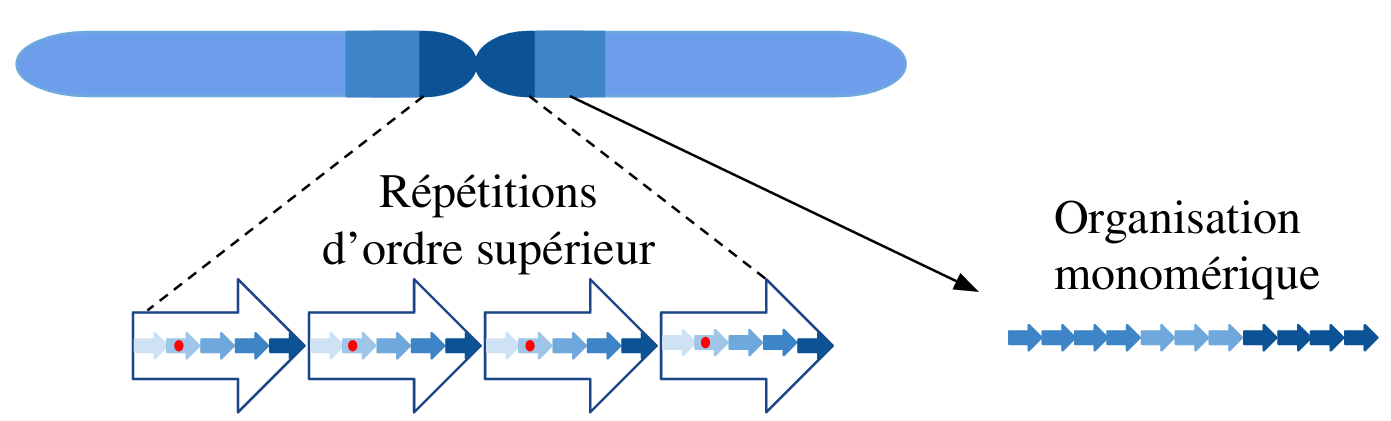
\includegraphics[height=3.5cm, width=12cm]{img/AS_organization.png}
		\caption{\textbf{Organisation spatiale des $\alpha$-satellites:} Le coeur du centromère (bleu foncé) est organisé en répétition d'ordre supérieur. Le péricentromère(bleu clair) a une organisation monomérique. Un monomère d'une même famille est représenté par une petite flèche de même couleur. Les points rouges représentent les sites de fixation à CENP-B ou pJ$\alpha$.}
\end{figure}


\subsection{Le sujet de stage}
enchaîne sur l'étude chez les cerco, une autre étude de séquençage haut débit\\

-travaux précédents limités (expliquer pk). Les méthodes basées aur l'alignement et la phylogénie sont très limitées, le jeu de données étant trop grand. Les méthodes n'étaient pas objectives (quelles méthodes??). De plus, chez d'autres espèces de Primates, les informations sont trop dispersées et aucune comparaison interespèce n'a été faite. \\


L'équipe d'accueil de mon stage "ADN répété, Chromatine, Evolution" ou ARChE, a récemment développé une approche de séquençage haut débit, ciblée sur les séquences $\alpha$-satellites chez deux espèces de Cercopithèques. Une autre étude avec un grand nombre de séquences concerne le Gorille [Catacchio] avec l'utilisation de fragments relativement longs. 

L'objectif de ce stage est de comprendre la fonction des $\alpha$-satellites et leur mécanisme d'évolution. Je vais choisir plusieurs espèces de Primates. Je vais utiliser une méthode de classification automatisée améliorée du laboratoire [Florence Jornod] pour classer les séquences en familles.  Ce programme permet de traiter des centaines de milliers de séquences sans quelque soit le nombre de séquences ou la taille des familles. Je vais dans un premier temps appliquer cette technologies au données issues de ce séquençage. Ensuite, je vais étudier d'autres espèces. Puisque toutes les espèces sont étudiées par la  même méthode, une comparaison inter espèce est envisageable. 

%%%%%%%%%%%%%%%%%%%%%%%%%%%%%%%%%%%%%%%%%%%%%%%%%%%%%%%%%%%%%%%%%
%%%%%%%%%%%%%%%%%%%%%%M & M%%%%%%%%%%%%%%%%%%%%%%%%%%%%%%%%%%%%%%
%%%%%%%%%%%%%%%%%%%%%%%%%%%%%%%%%%%%%%%%%%%%%%%%%%%%%%%%%%%%%%%%% 
\section{Matériel et méthode}
\subsection{Choix des espèces}
Les critères de sélection dépendent de la disponibilité des séquences de qualité. Deux espèces du laboratoire sont choisies, les \textit{Cercopithèques solatus} et \textit{pogonias}, et deux espèces proches, le \textit{Macaca fascicularis} et le \textit{Chlorocebus sabaeus}.  
	\begin{figure}
		\center
		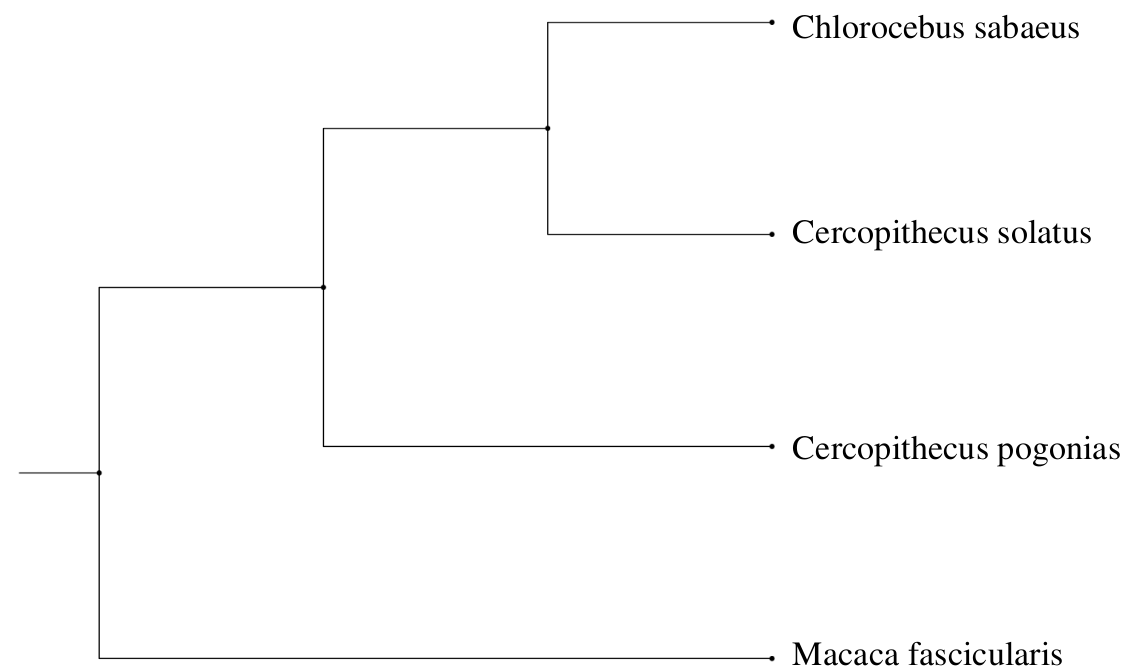
\includegraphics[height=4.5cm, width=7cm]{img/arbre_especes.png}
		\caption{\textbf{Arbre phylogénétique des espèces choisies.}}
	\end{figure}

\subsection{Méthode de classification}
Cette méthode \cite{rapport_florence} répartit des séquences $\alpha$-satellites en familles selon la similarité. La classification est hiérarchique dichotomique. Dans un premier temps, les séquences sont séparées en fonction de la fréquence des 5-mers qui composent les séquences, d'après les études sur les \textit{Cercopithèques}.

La classification est suivie d'une double validation des sous-groupes. D'une part la taille du sous-groupe est vérifiée. La taille minimale d'une famille est fixée à 100. Si un groupe atteint 100 séquences, il n'est pas redivisé. D'autre part les deux groupes doivent être distincts. Pour cela le \textit{matepair}, la proportion de monomères ayant son plus proche voisin dans le même groupe, est évalué. Des valeurs \textit{matepairs} élevées indiquent des sous-groupes bien homogènes et séparés validant la classification tandis qu’un seuil \textit{matepair} plus faible entraîne plus de classes. Si les \textit{matepairs} sont au-dessus d’un certain seuil, les deux sous-groupes sont ajoutés séparément à la file pour être potentiellement redivisés ultérieurement.En revanche, si au moins une des valeurs de \textit{matepair} est au dessous de ce seuil, les sous-groupes sont considérés comme formant un seul groupe et le groupe initial est sauvegardé comme une famille unique. 
	\begin{figure}
		\center
		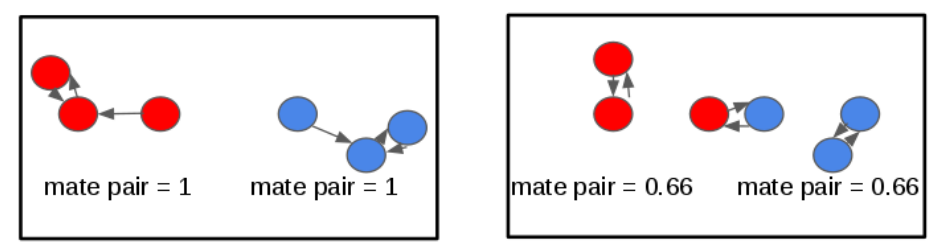
\includegraphics[height=2.5cm, width=8cm]{img/matepair.png}
		\caption{\textbf{Représentation du matepair:} Dans l'exemple de droite, les séquences "rouges" et les séquences "bleues" forment des groupent distincts. Leur pairmate est de 1. Dans l'exemple de droite, une séquence rouge est plus proche d'une séquence bleue, diminuant la valeur du pairmate à 0,66.}
	\end{figure}

La séparation des séquences se fait de façon itérative en boucle. Chaque tour implique une analyse en composante principale (ACP) et une classification hiérarchique. Si le jeu de données dépasse 110 000 séquences, le calcul des distances devient pesant. Une analyse discriminante linéaire (LDA) entre alors en jeu, avec un échantillon de taille 100 000. L'ACP est faite sur la table des 5-mers pour réduire les dimensions du jeu de données en minimisant la perte d'information et obtenir des variables indépendantes utilisables pour la LDA. Le nombre de composantes est fixé à 1024. Ensuite des distances euclidiennes sont calculées entre toutes les paires de séquences dans l’espace défini par les M premières composantes de l’ACP. Puis la méthode de classification hiérarchique de Ward forme des classes de façon à minimiser l’inertie interclasse. Cette méthode d'apprentissage utilise un sous-jeu de données formé par des séquences tirées aléatoirement. Le modèle construit est appliqué sur toutes les séquences.

\subsection{Alignement, consensus et phylogénie}
L'alignement des séquence est fait avec muscle \cite{muscle}. La phylogénie est reconstruite avec Seaview 
\cite{seaview} 
utilisant le modèle évolutif de Kimura à deux paramètre (K2P). L'arbre est construit avec l'algorithme  de Neighbor Joining (BioNJ) \cite{NJ}. Les consensus sont obtenus avec des scripts développés par l'équipe. Les motifs CENP-B (TTCGTTGGAA[AG]CGGGA), PJ$\alpha$ (TTCCTTTT[CT]CACC[AG]TAG) et pK$\beta$ (CTATAGGGCCAAAGGAA) ont été identifiés avec le logiciel fuzznuc (package EMBOSS) \cite{emboss} et en autorisant 2 différences au maximum par rapport au consensus. 

%%%%%%%%%%%%%%%%%%%%%%%%%%%%%%%%%%%%%%%%%%%%%%%%%%%%%%%%%%%%%%%%%
%%%%%%%%%%%%%%%%%%%%%%%%%%%%%%%%%%%%%%%%%%%%%%%%%%%%%%%%%%%%%%%%%
%%%%%%%%%%%%%%%%%%%%%%%%%%%%%%%%%%%%%%%%%%%%%%%%%%%%%%%%%%%%%%%%%
\section{Résultat}
	\subsection{Caractérisaton des familles dans plusieurs espèces}
			\subsubsection{Identification des familles}
			Les espèce \textit{C. solatus} et \textit{C. pogonias} sont analysés dans un premier temps pour comparer les résultats de la classification automatisée avec les résultats expérimentaux du laboratoire. Il existe 6 familles $\alpha$-satellites chez les \textit{Cercopithèques}. Ces deux espèces partagent deux grandes familles monomériques, C1 et C2, de l'ordre de plusieurs milliers de séquences. Elles partagent également le dimère C3-C4. \textit{C. pogonias} possède les familles supplémentaires C5 et C6.\\
			La classification automatisée donne des familles de tailles variables allant de deux  à des dizaines de milliers de séquences. Seules les familles ayant plus de 100 séquences, appelées "grandes familles", sont conservées pour l'analyse des familles. Les "petites familles" sont prises en compte en terme de pourcentage de séquences qui ne figurent pas dans l'analyse. Les séquences $\alpha$-satellites chez \textit{solatus} sont réparties en 564 familles, dont 12 grandes familles. Les séquences qui ne sont pas retenues représentent 3,97\% du jeu de données. Chez pogonias, le nombre total de familles est de 132, avec 13 grandes familles et 1,29\% du jeu de données qui  ne figure pas dans les analyses.\\
			 Le nombre de grandes familles est relativement proche entre ces deux espèces, mais diffèrent significativement des résultats expérimentaux. Parmi ces dizaines de familles, chez \textit{C. solatus} 11 familles forment la famille C2, une familles forme la famille C1 et les familles C3 et C4 sont retrouvées dans des petites familles d'environ 80 séquences chacune. Toutes les familles sont retrouvées chez \textit{C. pogonias} sauf la famille C6. La famille C1 est composée de 10 familles, les familles C2, C3 et C5 sont composé d'une famille respectivement, et C4 correspond a une petite famille. Ces résultats contredisent les résultats expérimentaux. La famille C2 et censée être divisée en plusieurs groupes par ses séquences qui divergent plus que dans la famille 1.  
			 La classification expérimentale est une méthode visuelle basée sur l'ACP sur des 5-mers. Un point noir représente un monomère. Deux groupes distincts regroupent les familles C1 et C2 chez solatus et 4 groupes distincts sont retrouvés chez pogonias formant les familles C1, C2, C5 et C6. Sur cette représentation sont superposées les familles de la classification automatisée en couleur. \\
			 Le \textit{C. sabaeus} a 338 familles au total, dont 44 grandes familles, et 10,89\% du jeu de données qui n'est pas pris en compte. Le \textit{M. fascicularis} a respectivement 709 et 998 familles, dont 42 et 81 grandes familles, et 14,56\% et 5,05\% du jeu de données qui n'est pas pris en compte. Ces espèces ont beaucoup plus de grandes familles que les \textit{Cercopithèques}. 
			 
	\begin{figure}	
		\begin{tabular}{cc} 
			\textbf{A.} & 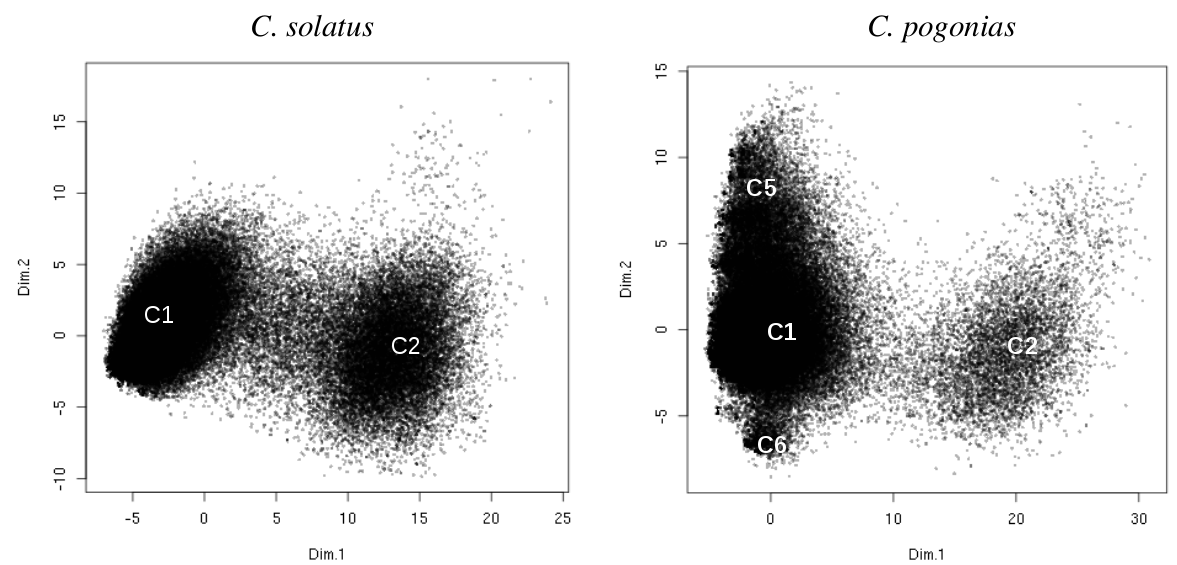
\includegraphics[scale=0.4]{img/ACP1.png}  \\
			\textbf{B.} & 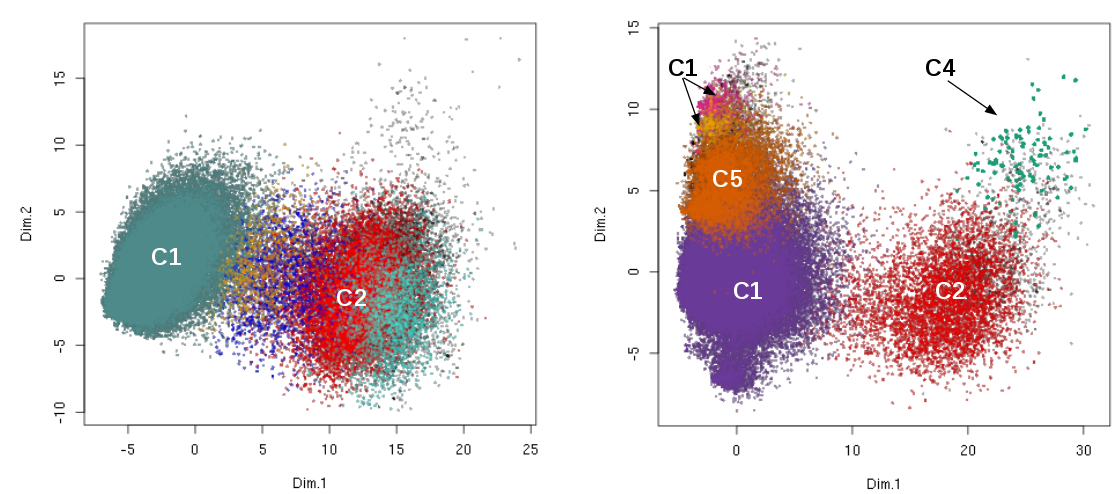
\includegraphics[scale=0.4]{img/ACP2.png}  \\
			\textbf{C.} & 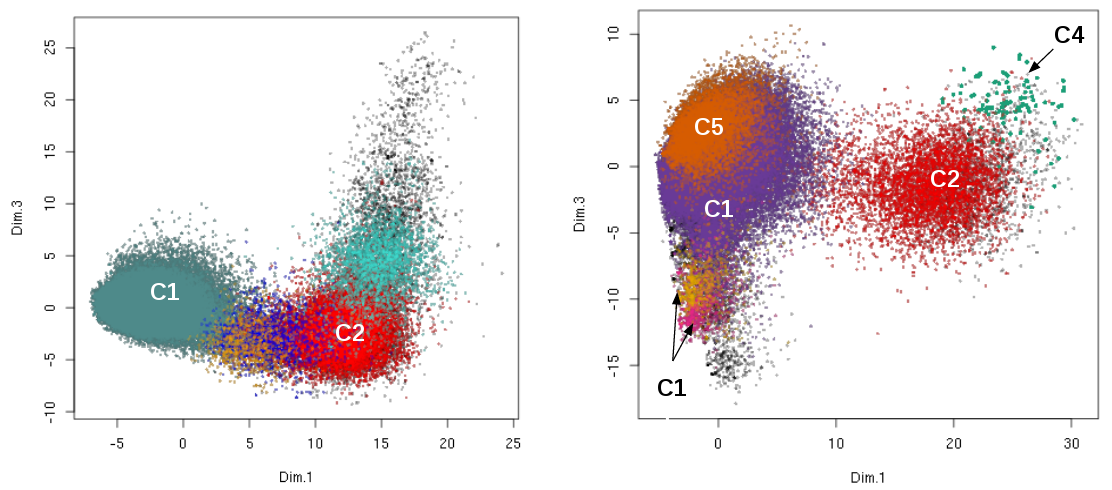
\includegraphics[scale=0.4]{img/ACP3.png}   \\
		\end{tabular}
\caption{\textbf{Représentation des ACP des 5-mers chez \textit{C. solatus} et \textit{C. pogonias}:}Les familles expérimentales C1 à C5 sont indiquées sur les graphiques. Chez solatus, les familles issues de la classification automatisée sont C1 en darkslategray4 et C2 en rouge, blue, turquoise, orange. Chez pogonias, C1 est en violet, jaune et rose; C2 est en rouge; C4 est en vert; C5 est en orange.\textbf{A.} Classification expérimentale. Un monomère est représenté par un point noir. \textbf{B.} Représentation des composantes 1 et 2 de l'ACP. \textbf{C.} Représentation des composantes 1 et 3 de l'ACP..} 
\end{figure}
		
			\subsubsection{Motifs CENP-B, pJ$\alpha$ et pK$\beta$}
			\subsubsection{Similarité entre familles}
	
	\subsection{Comparaison inter-espèce et mécanismes d'évolution}
		\subsubsection{Résultats du laboratoire}
		Le laboratoire a effectué un séquençage sur les \textit{C. solatus} et \textit{pogonias}. Les séquences $\alpha$-satellites obtenues sont divisées en nucléotides de 5-mers, puis triées par Analyse de Classification Hiérarchique (HCA) et par Analyse Discriminante Linéaire (LDA). Chez le \textit{C. solatus}[article 1 de Laurianne] deux grandes familles monomériques (C1 et C2) et un HOR d'ordre 2, composé des familles C3 et C4, sont identifiés. Chez le \textit{C. pogonias}[article2 de Laurianne], deux familles supplémentaires (C5 et C6) ont été détectées. Ces \textit{Cercopithèques} ne disposent pas du site de fixation pour la protéine CENP-B. Au contraire, le site de fixation pour la protéine pJ$\alpha$ est présent dans 85\% des $\alpha$-satellites en moyenne, excepté la famille C3 qui n'en possède pas.  
		\subsubsection{Comparaison des familles}
		
Le programme identifie 13 et 14 familles chez le \textit{C. solatus} et \textit{pogonias} respectivement. Seules les familles de plus de 100 séquences sont conservées. Cette sélection implique 6,99\% et 1.63\% en perte d'information pour ces deux espèces. Les séquences restantes, n'ayant pas été classées dans une famille assez grande ou étant peut-être des séquences atypiques, ne sont pas prises en compte dans l'analyse. 

Le \textit{C.solatus} a deux grandes familles de 82911 et 9216 monomères, une classe intermédiaire de 1519,1267 et 898 séquences. Le \textit{C.pogonias} a 3 grandes familles d'$\alpha$-satellites qui ont 94594, 8319 et 5202 séquences, deux familles intermédiaires de 998 et 664 monomères. Les familles restantes ont quelques centaines de séquences et sont très petites comparées au familles citées ci-dessus. Une ACP permet de visualiser et de comparer les familles (Figure 2). 

La famille C1 est divisée en plusieurs familles pour les deux espèces.La famille C2 péricentromérique est retrouvée chez les deux espèces et forme un complexe homogène. Les dimères sont une famille d'une centaine de monomères. La famille C3 est retrouvée chez le \textit{C.pogonias} seulement, bien qu'elle n'ait pas été étudiée dans les études du \textit{C.pogonias}. La famille C4 n'est pas détectée. Cette famille a probablement été divisée en petites classes. Elles ne sont donc pas détectées. La famille C5 est retrouvée. C6 et C1 ont été classé comme étant une même famille. 

%\begin{figure}
%	\center
%		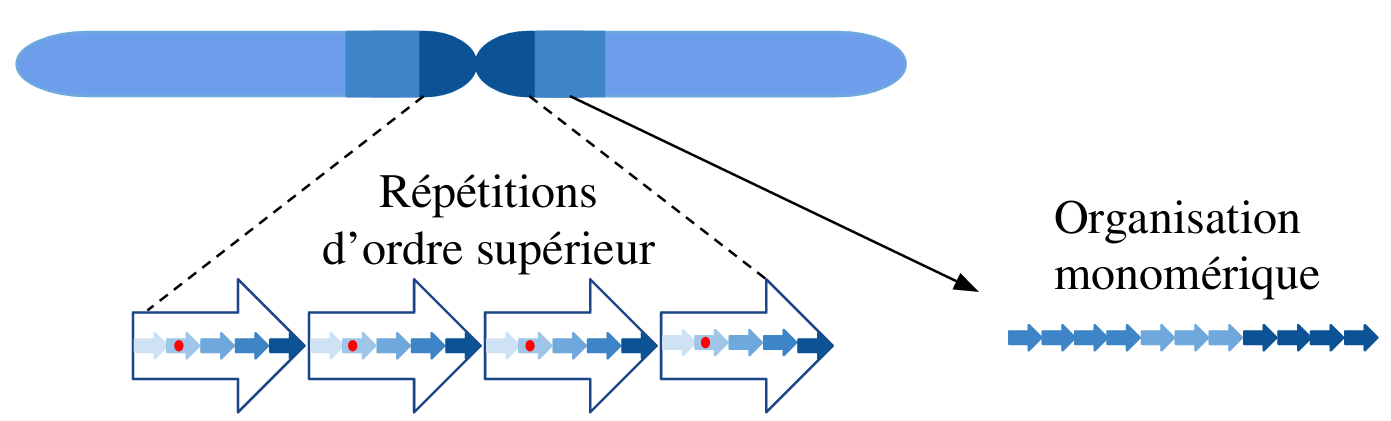
\includegraphics[height=3.5cm, width=12cm]{img/AS_organization.png}
%		\caption{\textbf{Organisation spatiale des $\alpha$-satellites:} Le coeur du centromère (bleu foncé) est organisé en répétition d'ordre supérieur. Le péricentromère(bleu clair) a une organisation monomérique. Un monomère d'une même famille est représenté par une petite flèche de même couleur. Les points rouges représentent les sites de fixation à CENP-B ou pJ$\alpha$.}
%\end{figure}
\begin{figure}	
\begin{tabular}{cc}
% \hspace*{0.5cm} &  
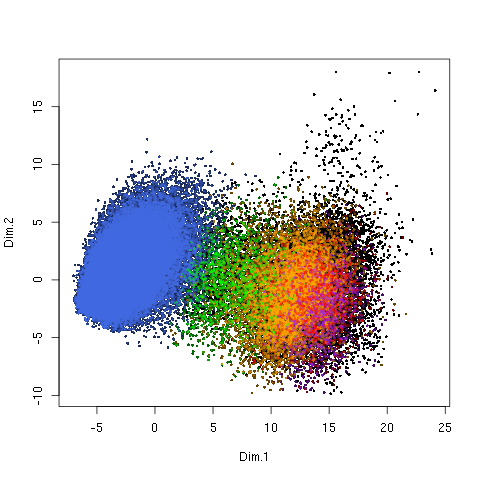
\includegraphics[scale=0.5]{img/Cso_acp_pm090_rapport.png}
\end{tabular}
\hfill
\begin{tabular}{c}
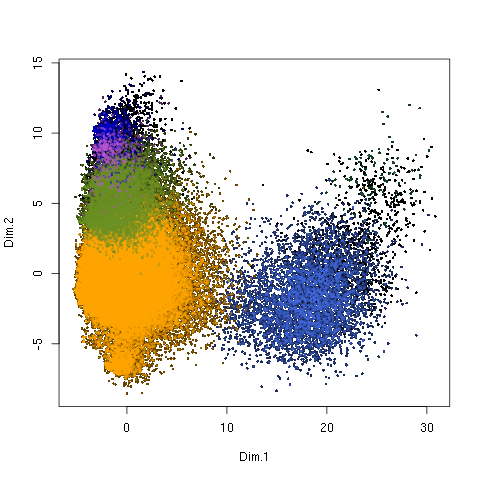
\includegraphics[scale=0.5]{img/Cp_acp_pm090_rapport.png}
\end{tabular}
%\hspace*{1cm}
\caption{ACP des 5-mers chez \textit{C.solatus} (à gauche) et \textit{C.pogonias} (à droite) : Les familles communes sont C1 (orange) et C2 (royalblue).  C3 (seagreen) et C5 (olivedrab) sont visibles seulement chez pogonias. Les familles qui divisent C1 sont la 2 (green), 73 (red) et 177 (purple)et chez pogonias la 11 (mediumblue) et 51 (mediumorchid).} 
\end{figure}

\section{Discussion}
\section{Conclusion}
\bibliographystyle{plain} \bibliography{biblio} 

%
%	\makeindex % index général
%   \newindex{env}{enx}{end}{Environnements}
%   \newindex{ext}{exx}{exd}{Extensions}
%   \newindex{cmm}{cmx}{cmd}{Commandes}
%	\newcommand{\commande}[1]
%   {\texttt{\textbackslash #1}}
%	\newcommand{\indexcmm}[1]
%   {\index[cmm]{#1@\commande{#1}}} % index d'une commande
% 
%
%
%
%Une citation\index{citation} hors paragraphe
%se met dans un environnement
%\emph{quote}\index[env]{quote}
%ou \emph{quotation}\index[env]{quotation}
% 
%L'extension \emph{array}\index[ext]{array}
%fournit les commandes
%\commande{raggedleft}\indexcmm{raggedleft}
%et \commande{raggedright}\indexcmm{raggedright}.
% 
%\printindex % index général
%\printindex[env]
%\printindex[ext]
%\printindex[cmm]

%%%%%%%%%%%%%%%%%%%%%%%%%%%%%%%%%%%%%%%%%%%%%%%%%%%%%%%%%%%%%%%%%%
%%%%%%%%%%%%%%%%%%%%Résumé & Abstract%%%%%%%%%%%%%%%%%%%%%%%%%%%%%
%%%%%%%%%%%%%%%%%%%%%%%%%%%%%%%%%%%%%%%%%%%%%%%%%%%%%%%%%%%%%%%%%%
\newpage 
\thispagestyle{empty}
\section*{Résumé}~\\[0.2cm]
Votre résumé commence ici...
   ...
\section*{Abstract}~\\[0.2cm]
 Abstract begins here...
   ...
\end{document}
%
%%HELP: http://lataix-sebastien.developpez.com/tutoriels/latex/memoire-de-fin-d-etude/#LII-C